%==============================================================================
% Tento soubor použijte jako základ
% This file should be used as a base for the thesis
% Autoři / Authors: 2008 Michal Bidlo, 2022 Jaroslav Dytrych
% Kontakt pro dotazy a připomínky: sablona@fit.vutbr.cz
% Contact for questions and comments: sablona@fit.vutbr.cz
%==============================================================================
% kódování: UTF-8 (zmena prikazem iconv, recode nebo cstocs)
% encoding: UTF-8 (you can change it by command iconv, recode or cstocs)
%------------------------------------------------------------------------------
% zpracování / processing: make, make pdf, make clean
%==============================================================================
% Soubory, které je nutné upravit nebo smazat: / Files which have to be edited or deleted:
%   projekt-20-literatura-bibliography.bib - literatura / bibliography
%   projekt-01-kapitoly-chapters.tex - obsah práce / the thesis content
%   projekt-01-kapitoly-chapters-en.tex - obsah práce v angličtině / the thesis content in English
%   projekt-30-prilohy-appendices.tex - přílohy / appendices
%   projekt-30-prilohy-appendices-en.tex - přílohy v angličtině / appendices in English
%==============================================================================
\documentclass[]{fitthesis} % bez zadání - pro začátek práce, aby nebyl problém s překladem
%\documentclass[english]{fitthesis} % without assignment - for the work start to avoid compilation problem
%\documentclass[zadani]{fitthesis} % odevzdani do IS VUT a/nebo tisk s barevnými odkazy - odkazy jsou barevné
%\documentclass[english,zadani]{fitthesis} % for submission to the IS VUT and/or print with color links - links are color
%\documentclass[zadani,print]{fitthesis} % pro černobílý tisk - odkazy jsou černé
%\documentclass[english,zadani,print]{fitthesis} % for the black and white print - links are black
%\documentclass[zadani,cprint]{fitthesis} % pro barevný tisk - odkazy jsou černé, znak VUT barevný
%\documentclass[english,zadani,cprint]{fitthesis} % for the print - links are black, logo is color
% * Je-li práce psaná v anglickém jazyce, je zapotřebí u třídy použít 
%   parametr english následovně:
%   If thesis is written in English, it is necessary to use 
%   parameter english as follows:
%      \documentclass[english]{fitthesis}
% * Je-li práce psaná ve slovenském jazyce, je zapotřebí u třídy použít 
%   parametr slovak následovně:
%   If the work is written in the Slovak language, it is necessary 
%   to use parameter slovak as follows:
%      \documentclass[slovak]{fitthesis}
% * Je-li práce psaná v anglickém jazyce se slovenským abstraktem apod., 
%   je zapotřebí u třídy použít parametry english a enslovak následovně:
%   If the work is written in English with the Slovak abstract, etc., 
%   it is necessary to use parameters english and enslovak as follows:
%      \documentclass[english,enslovak]{fitthesis}

% Základní balíčky jsou dole v souboru šablony fitthesis.cls
% Basic packages are at the bottom of template file fitthesis.cls
% zde můžeme vložit vlastní balíčky / you can place own packages here


% Pro seznam zkratek lze využít balíček Glossaries - nutno odkomentovat i níže a při kompilaci z konzoly i v Makefile (plnou verzi pro Perl, nebo lite)
% The Glossaries package can be used for the list of abbreviations - it is necessary to uncomment also below. When compiling from the console also in the Makefile (full version for Perl or lite)
%\usepackage{glossaries}
%\usepackage{glossary-superragged}
%\makeglossaries 

% Nastavení cesty k obrázkům
% Setting of a path to the pictures
%\graphicspath{{obrazky-figures/}{./obrazky-figures/}}
%\graphicspath{{obrazky-figures/}{../obrazky-figures/}}

%---rm---------------
\renewcommand{\rmdefault}{lmr}%zavede Latin Modern Roman jako rm / set Latin Modern Roman as rm
%---sf---------------
\renewcommand{\sfdefault}{qhv}%zavede TeX Gyre Heros jako sf
%---tt------------
\renewcommand{\ttdefault}{lmtt}% zavede Latin Modern tt jako tt

% vypne funkci šablony, která automaticky nahrazuje uvozovky,
% aby nebyly prováděny nevhodné náhrady v popisech API apod.
% disables function of the template which replaces quotation marks
% to avoid unnecessary replacements in the API descriptions etc.
\csdoublequotesoff

\usepackage{url}
\usepackage{amsthm}
\usepackage{tikz}
\usepackage{pgfplots}
\usepackage{caption}
\pgfplotsset{compat = newest}

% =======================================================================
% balíček "hyperref" vytváří klikací odkazy v pdf, pokud tedy použijeme pdflatex
% problém je, že balíček hyperref musí být uveden jako poslední, takže nemůže
% být v šabloně
% "hyperref" package create clickable links in pdf if you are using pdflatex.
% Problem is that this package have to be introduced as the last one so it 
% can not be placed in the template file.
\ifWis
\ifx\pdfoutput\undefined % nejedeme pod pdflatexem / we are not using pdflatex
\else
  \usepackage{color}
  \usepackage[unicode,colorlinks,hyperindex,plainpages=false,pdftex]{hyperref}
  \definecolor{hrcolor-ref}{RGB}{223,52,30}
  \definecolor{hrcolor-cite}{HTML}{2F8F00}
  \definecolor{hrcolor-urls}{HTML}{092EAB}
  \hypersetup{
	linkcolor=hrcolor-ref,
	citecolor=hrcolor-cite,
	filecolor=magenta,
	urlcolor=hrcolor-urls
  }
  \def\pdfBorderAttrs{/Border [0 0 0] }  % bez okrajů kolem odkazů / without margins around links
  \pdfcompresslevel=9
\fi
\else % pro tisk budou odkazy, na které se dá klikat, černé / for the print clickable links will be black
\ifx\pdfoutput\undefined % nejedeme pod pdflatexem / we are not using pdflatex
\else
  \usepackage{color}
  \usepackage[unicode,colorlinks,hyperindex,plainpages=false,pdftex,urlcolor=black,linkcolor=black,citecolor=black]{hyperref}
  \definecolor{links}{rgb}{0,0,0}
  \definecolor{anchors}{rgb}{0,0,0}
  \def\AnchorColor{anchors}
  \def\LinkColor{links}
  \def\pdfBorderAttrs{/Border [0 0 0] } % bez okrajů kolem odkazů / without margins around links
  \pdfcompresslevel=9
\fi
\fi
% Řešení problému, kdy klikací odkazy na obrázky vedou za obrázek
% This solves the problems with links which leads after the picture
%\usepackage[all]{hypcap}


% Informace o práci/projektu / Information about the thesis
%---------------------------------------------------------------------------
\projectinfo{
  %Prace / Thesis
  project={BP},            %typ práce BP/SP/DP/DR  / thesis type (SP = term project)
  year={2024},             % rok odevzdání / year of submission
  date=\today,             % datum odevzdání / submission date
  %Nazev prace / thesis title
  title.cs={Fuzzy implikace},  % název práce v češtině či slovenštině (dle zadání) / thesis title in czech language (according to assignment)
  title.en={Fuzzy implications}, % název práce v angličtině / thesis title in english
  %title.length={14.5cm}, % nastavení délky bloku s titulkem pro úpravu zalomení řádku (lze definovat zde nebo níže) / setting the length of a block with a thesis title for adjusting a line break (can be defined here or below)
  %sectitle.length={14.5cm}, % nastavení délky bloku s druhým titulkem pro úpravu zalomení řádku (lze definovat zde nebo níže) / setting the length of a block with a second thesis title for adjusting a line break (can be defined here or below)
  %dectitle.length={14.5cm}, % nastavení délky bloku s titulkem nad prohlášením pro úpravu zalomení řádku (lze definovat zde nebo níže) / setting the length of a block with a thesis title above declaration for adjusting a line break (can be defined here or below)
  %Autor / Author
  author.name={Veronika},   % jméno autora / author name
  author.surname={Jirmusová},   % příjmení autora / author surname 
  %author.title.p={Bc.}, % titul před jménem (nepovinné) / title before the name (optional)
  %author.title.a={Ph.D.}, % titul za jménem (nepovinné) / title after the name (optional)
  %Ustav / Department
  department={UITS}, % doplňte příslušnou zkratku dle ústavu na zadání: UPSY/UIFS/UITS/UPGM / fill in appropriate abbreviation of the department according to assignment: UPSY/UIFS/UITS/UPGM
  % Školitel / supervisor
  supervisor.name={Dana},   % jméno školitele / supervisor name 
  supervisor.surname={Hliněná},   % příjmení školitele / supervisor surname
  supervisor.title.p={doc. RNDr.},   %titul před jménem (nepovinné) / title before the name (optional)
  supervisor.title.a={Ph.D.},    %titul za jménem (nepovinné) / title after the name (optional)
  % Klíčová slova / keywords
  keywords.cs={Sem budou zapsána jednotlivá klíčová slova v českém (slovenském) jazyce, oddělená čárkami.}, % klíčová slova v českém či slovenském jazyce / keywords in czech or slovak language
  keywords.en={Sem budou zapsána jednotlivá klíčová slova v anglickém jazyce, oddělená čárkami.}, % klíčová slova v anglickém jazyce / keywords in english
  %keywords.en={Here, individual keywords separated by commas will be written in English.},
  % Abstrakt / Abstract
  abstract.cs={Do tohoto odstavce bude zapsán výtah (abstrakt) práce v českém (slovenském) jazyce.}, % abstrakt v českém či slovenském jazyce / abstract in czech or slovak language
  abstract.en={Do tohoto odstavce bude zapsán výtah (abstrakt) práce v anglickém jazyce.}, % abstrakt v anglickém jazyce / abstract in english
  %abstract.en={An abstract of the work in English will be written in this paragraph.},
  % Prohlášení (u anglicky psané práce anglicky, u slovensky psané práce slovensky; u projektové praxe lze zakomentovat) / Declaration (for thesis in english should be in english; for project practice can be commented out)
  declaration={Prohlašuji, že jsem tuto bakalářskou práci vypracoval samostatně pod vedením pana X...
Další informace mi poskytli...
Uvedl jsem všechny literární prameny, publikace a další zdroje, ze kterých jsem čerpal.},
  %declaration={I hereby declare that this Bachelor's thesis was prepared as an original work by the author under the supervision of Mr. X
% The supplementary information was provided by Mr. Y
% I have listed all the literary sources, publications and other sources, which were used during the preparation of this thesis.},
  % Poděkování (nepovinné, nejlépe v jazyce práce; nechcete-li, zakomentujte pro skrytí nadpisu) / Acknowledgement (optional, ideally in the language of the thesis; comment out for hiding including heading)
  acknowledgment={V této sekci je možno uvést poděkování vedoucímu práce a těm, kteří poskytli odbornou pomoc
(externí zadavatel, konzultant apod.).},
  %acknowledgment={Here it is possible to express thanks to the supervisor and to the people which provided professional help
%(external submitter, consultant, etc.).},
  % Rozšířený abstrakt (cca 3 normostrany) - lze definovat zde nebo níže / Extended abstract (approximately 3 standard pages) - can be defined here or below
  %extendedabstract={Do tohoto odstavce bude zapsán rozšířený výtah (abstrakt) práce v českém (slovenském) jazyce.},
  %extabstract.odd={true}, % Začít rozšířený abstrakt na liché stránce? / Should extended abstract start on the odd page?
  %faculty={FIT}, % FIT/FEKT/FSI/FA/FCH/FP/FAST/FAVU/USI/DEF
  faculty.cs={Fakulta informačních technologií}, % Fakulta v češtině - pro využití této položky výše zvolte fakultu DEF / Faculty in Czech - for use of this entry select DEF above
  faculty.en={Faculty of Information Technology}, % Fakulta v angličtině - pro využití této položky výše zvolte fakultu DEF / Faculty in English - for use of this entry select DEF above
  department.cs={Ústav matematiky}, % Ústav v češtině - pro využití této položky výše zvolte ústav DEF nebo jej zakomentujte / Department in Czech - for use of this entry select DEF above or comment it out
  department.en={Institute of Mathematics} % Ústav v angličtině - pro využití této položky výše zvolte ústav DEF nebo jej zakomentujte / Department in English - for use of this entry select DEF above or comment it out
}

% Rozšířený abstrakt (cca 3 normostrany) - lze definovat zde nebo výše / Extended abstract (approximately 3 standard pages) - can be defined here or above
%\extendedabstract{Do tohoto odstavce bude zapsán výtah (abstrakt) práce v českém (slovenském) jazyce.}
% Začít rozšířený abstrakt na liché stránce? / Should extended abstract start on the odd page?
%\extabstractodd{true}

% nastavení délky bloku s titulkem pro úpravu zalomení řádku - lze definovat zde nebo výše / setting the length of a block with a thesis title for adjusting a line break - can be defined here or above
%\titlelength{14.5cm}
% nastavení délky bloku s druhým titulkem pro úpravu zalomení řádku - lze definovat zde nebo výše / setting the length of a block with a second thesis title for adjusting a line break - can be defined here or above
%\sectitlelength{14.5cm}
% nastavení délky bloku s titulkem nad prohlášením pro úpravu zalomení řádku - lze definovat zde nebo výše / setting the length of a block with a thesis title above declaration for adjusting a line break - can be defined here or above
%\dectitlelength{14.5cm}

% řeší první/poslední řádek odstavce na předchozí/následující stránce
% solves first/last row of the paragraph on the previous/next page
\clubpenalty=10000
\widowpenalty=10000

% checklist
\newlist{checklist}{itemize}{1}
\setlist[checklist]{label=$\square$}

% Kompilace po částech (rychlejší, ale v náhledu nemusí být vše aktuální)
% Compilation piecewise (faster, but not all parts in preview will be up-to-date)
% Další informace viz / For more information see https://www.overleaf.com/learn/latex/Multi-file_LaTeX_projects
% \usepackage{subfiles}

% Nechcete-li, aby se u oboustranného tisku roztahovaly mezery pro zaplnění stránky, odkomentujte následující řádek / If you do not want enlarged spacing for filling of the pages in case of duplex printing, uncomment the following line
% \raggedbottom

\begin{document}
  % Vysazeni titulnich stran / Typesetting of the title pages
  % ----------------------------------------------
  \maketitle
  % Obsah
  % ----------------------------------------------
  \setlength{\parskip}{0pt}

  {\hypersetup{hidelinks}\tableofcontents}
  
  % Seznam obrazku a tabulek (pokud prace obsahuje velke mnozstvi obrazku, tak se to hodi)
  % List of figures and list of tables (if the thesis contains a lot of pictures, it is good)
  \ifczech
    \renewcommand\listfigurename{Seznam obrázků}
  \fi
  \ifslovak
    \renewcommand\listfigurename{Zoznam obrázkov}
  \fi
  {\hypersetup{hidelinks}\listoffigures}
  
  \ifczech
    \renewcommand\listtablename{Seznam tabulek}
  \fi
  \ifslovak
    \renewcommand\listtablename{Zoznam tabuliek}
  \fi
   {\hypersetup{hidelinks}\listoftables}

  % Seznam zkratek / List of abbreviations
  %\ifczech
  %  \renewcommand*\glossaryname{Seznam zkratek}%
  %  \renewcommand*\entryname{Zkratka}
  %  \renewcommand*\descriptionname{Význam}
  %\fi
  %\ifslovak
  %  \renewcommand*\glossaryname{Zoznam skratiek}%
  %  \renewcommand*\entryname{Skratka}
  %  \renewcommand*\descriptionname{Význam}
  %\fi
  %\ifenglish
  %  \renewcommand*\glossaryname{List of abbreviations}%
  %  \renewcommand*\entryname{Abbreviation}
  %  \renewcommand*\descriptionname{Meaning}
  %\fi
  % Definice zkratek - z textu se odkazují např. \Gls{TF–IDF}
  % Definition of abbreviations - referred from the text e.g. \Gls{TF–IDF}
  %\newglossaryentry{TF–IDF}
  %{
  %  name={TF–IDF},
  %  description={Term Frequency-Inverse Document Frequency}
  %}
  % 
  %\setglossarystyle{superragged}
  %\printglossaries


  \ifODSAZ
    \setlength{\parskip}{0.5\bigskipamount}
  \else
    \setlength{\parskip}{0pt}
  \fi

  % vynechani stranky v oboustrannem rezimu
  % Skip the page in the two-sided mode
  \iftwoside
    \cleardoublepage
  \fi

  % Text prace / Thesis text
  % ----------------------------------------------
  \ifenglish
    \input{projekt-01-kapitoly-chapters-en}
  \else
    % Tento soubor nahraďte vlastním souborem s obsahem práce.
%=========================================================================
% Autoři: Michal Bidlo, Bohuslav Křena, Jaroslav Dytrych, Petr Veigend a Adam Herout 2019

% Pro kompilaci po částech (viz projekt.tex), nutno odkomentovat a upravit
%\documentclass[../projekt.tex]{subfiles}

%\newenvironment{definice}{\begin{quote}\textbf{Definice:}}{\end{quote}}

\newtheorem{definition}{Definice}
\newtheorem{remark}{Pozn\'amka}
\newtheorem{example}{Příklad}
\newtheorem{graph}{Obr\' azek}
\newcommand{\comment}[1]{}

\chapter{Úvod}

\color{blue} Pár vět, které pak chci zakomponovat do \'uvodu nějak:
                \\ 
                \color{black} Zatímco bivalenční logika pracuje s binárními hodnotami "pravda" a "nepravda", fuzzy logika umožňuje pracovat s hodnotami, které se pohybují mezi těmito extrémy.


\chapter{Abstrakt}
\label{abstrakt}




\chapter {Fuzzy mno\v ziny a fuzzy logika}
\section{Fuzzy mno\v ziny} 

\comment{
V klasické i fuzzy logice se často setkáváme se základními pojmy množina a prvek množiny. Množina se obecně vysvětluje jako souhrn, soubor nebo skupina objektů. Tyto objekty pak nazýváme prvky dané množiny. Nejvíce charakteristická vlastnost množin je, že je jednoznačně určena svými prvky, ale ignoruje jejich pořadí a další jejich struktury. Množina, která neobsahuje žádné prvky, se nazývá prázdná množina.
}

V běžném životě se často setkáváme s nepřesnými pojmy, jako jsou např. \clqq málo\crqq, \clqq hodně\crqq \space či třeba \clqq trochu\crqq \space. Jak ale takovou vágnost vyjádřit v matematice? Pokud člověk vyjádří výrok, že je \clqq celkem mladý\crqq, znamená to, že je mladý nebo ne? K zápisu a práci s takovými výroky se pak ve fuzzy logice využívají fuzzy množiny a operace s nimi.

Nech\v t je např. vypsáno výběrové řízení modelingové agentury s požadavkem, že hledají vysoké uchazeče. Taková informace je tedy poněkud vágní, ačkoliv v běžném životě lehce srozumitelná. Pokud by se někdo pokusil definovat pojem \clqq vysoký člověk\crqq \space pomocí ostré množiny, musel by nejprve stanovit hranici, kdy je člověk vysoký, např. 180 centimetr\r u, množina všech vysokých lidí V by měla charakteristickou funkci

    $$\chi_V:(x)=\begin{cases} 1, & \mbox{pokud }  x \geq 180\\    0, & \mbox{pokud } x < 180,  \end{cases}$$

    čímž by došlo k paradoxu, že člověk který má 179,9 centimetr\r u je považován za nízkého a člověk se 180 centimetry za vysokého.

    Takový problém je zp\r usoben tím, že byla výška modelována jako vlastnost, kterou m\r uže mít člověk pouze v nulové míře nebo na 100\%. Za určitě vysokého člověka byl považován někdo se 180 centimetry, 175 centimetr\r u vysoký člověk byl podle stejného přístupu určitě malý. Přičemž 175 centimetr\r u vysoký člověk je běžně považován do určité míry za vysokého. Přesně z toho d\r uvodu se zavedl pojem \textit{fuzzy množina}. 
    \begin{definition}
    \cite{navara}
        Fuzzy podmnožina univerza X (stručně fuzzy množina) je objekt A, který popisuje (zobecněná) charakteristická funkce (funkce příslušnosti) $\mu: X \rightarrow [0,1]$. Obor pravdivostních hodnot: $R(A) = \{\alpha \in [0,1]: (\exists x \in X : \mu_A(x) = \alpha)\} = \mu_A(X)$
    \end{definition}
    Fuzzy množina nebo také neostrá množina je pak množina prvků takových, jejichž afiliace je k této množině odstupňovaná. Fuzzy množina staví na stejných pravidlech, jako klasická booleovská množina, s tím rozdílem, že příslušnost nemusí nabývat jen hodnot 0 a 1, ale jakoukoliv hodnotu z intervalu [0,1].
    
    Ve fuzzy matematice se dále zavedl pojem Funkce příslušnosti.
    \begin{definition}
        \cite{Kolo} Funkce příslušnosti fuzzy množiny A na (ostré) množině X: $\mu_A : X \rightarrow  [0,1].$ Stupe\v n příslušnosti x $\in A$ tedy m\r uže být libovolné číslo $\alpha \in [0,1]$.
    \end{definition}
    Funkce příslušnosti umož\v nuje vyjádřit částečnou příslušnost k množinám na intervalu [0,1], tedy jak moc lze označit pojem za \clqq pravdu\crqq \space či \clqq nepravdu\crqq. Díky čemuž se pak dají matematicky vyjádřit vágní pojmy jako \clqq docela dost\crqq, \clqq málo\crqq \space nebo \clqq mnoho\crqq \space apod.

     Pokud by se v předchozím zmíněném výběru modelingové agentury označila výška 180 centimetr\r u stupněm vlastnosti \clqq vysoký\crqq \space 1, pak je možné přiřadit výšce 175 cemtimetr\r u například stupe\v n 0,85. Když je každému prvku $x$ ze základního prostoru [0, $\infty$[ přiřazeno číslo z intervalu [0,1], které vyjadřuje míru, ve které je člověk mající výšku $x$ vysoký, lze pak získat funkci, která kompletně charakterizuje pojem vysoký člověk: $\mu_V: \Omega \rightarrow [0,1]$, kde $\Omega = [0, \infty[$ vyjadřuje základní prostor neboli univerzum. Takovou funkcí je např. funkce $\mu_V:  [0, \infty[ \rightarrow [0,1]$, 

    $$\mu_V:(x)=\begin{cases} 1, & \mbox{pokud }  x \geq 180\\ 
    \frac{x}{20} - 8, & \mbox{pokud } 160 \leq x \leq 180\\
    0, & \mbox{pokud } x < 160,  \end{cases}$$

    jíž graf je vykreslen níže.

    \begin{graph} Graf funkce příslušnosti fuzzy množiny V - \clqq Vysoký člověk\crqq.\\
        \begin{tikzpicture}
        \hspace*{2cm}
            \begin{axis}[
                xlabel=$x$, % Popisek osy x
                ylabel=$\mu_V(x)$, % Popisek osy y
                axis lines=middle, % Zobrazení os
                ymin=0, ymax=1,2, % Rozsah osy y
                xmin=0, xmax=250, % Rozsah osy x
                xtick={0, 160, 180}, % Označení na ose x
                ytick={ 0, 0.8, 1}, % Označení na ose y
                legend style={at={(0.5,-0.2)}, anchor=north},
                width=10cm, % Šířka grafu
                height=6cm, % Výška grafu
                grid=both, % Zobrazení mřížky
                grid style={line width=0.2pt, draw=gray!30},
            ]
            
            % Definice prvního segmentu
            \addplot[blue, ultra thick, domain=180:250, samples=100] {1};
            
            % Definice druhého segmentu
            \addplot[blue, ultra thick, domain=160:180, samples=100] {x/20 - 8};
             \addlegendentry{V}
            
            % Definice třetího segmentu
            \addplot[blue, ultra thick, domain=0:160, samples=100] {0};
            
            \end{axis}
        \end{tikzpicture}
    \end{graph}



Pokud bychom chtěli modelovat funkci příslušnosti odlišného fuzzy výroku, např. výroku \clqq asi 3\crqq, lze zvolit několik možných řešení tohoto problému. Každý pak vyjadřuje jiný rozptyl možných řešení.
\begin{graph} Grafické znázornění funkcí příslušnosti výroku P \clqq asi 3\crqq.\\


    \resizebox{150pt}{!}{%zde se meni velikost grafu
                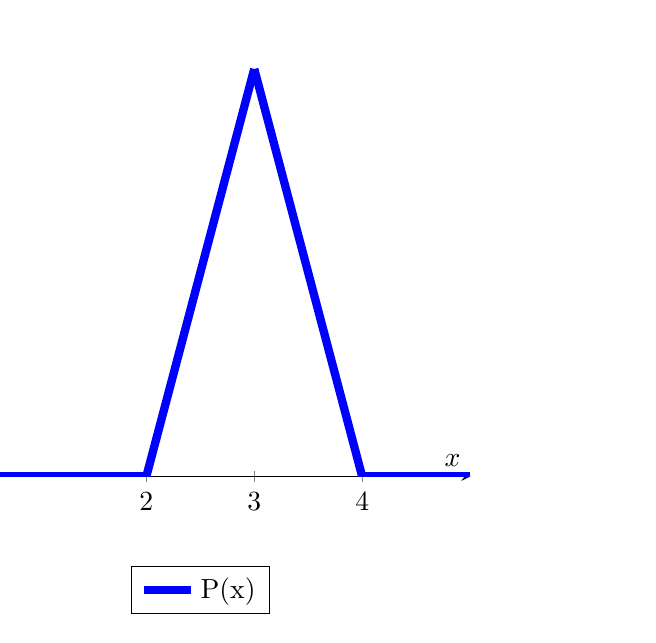
\begin{tikzpicture}
                \hspace*{-2cm}
                	\begin{axis}[
                        axis lines=middle,
                        xlabel=$x$,
                        ylabel=$y$,
                        xtick={0, 2, 3, 4}, % Označení na ose x
                        ytick={ 0, 0.5, 0.8, 1}, % Označení na ose y
                        legend style={at={(0.5,-0.2)}, anchor=north},
                        xmin=0, xmax=5, 
                        ymin=0, ymax=1.1,
                    ]
                    
                    \addplot[blue, domain=0:3, line width = 3pt] {x-2};
                    \addlegendentry{P(x)}
                    
                    \addplot[blue, domain=3:5, line width = 3pt,] {-x + 4};
                    \addplot[blue, domain=4:5, line width = 3pt,] {0};
                    \addplot[blue, domain=0:2, line width = 3pt,] {0};

                	\end{axis}
                \end{tikzpicture}
            }
            \resizebox{150pt}{!}{%zde se meni velikost grafu
                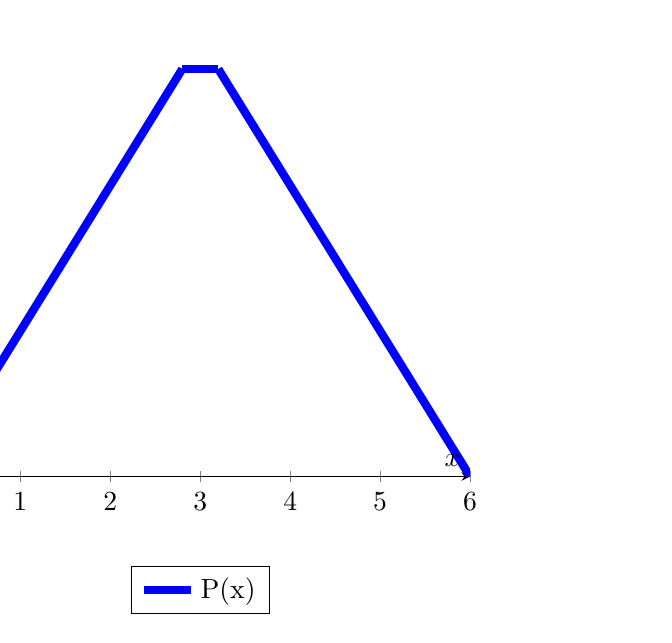
\begin{tikzpicture}
                \hspace*{-2cm}
                	\begin{axis}[
                        axis lines=middle,
                        xlabel=$x$,
                        ylabel=$y$,
                        xtick={0, 1, 2, 3, 4, 5, 6}, % Označení na ose x
                        ytick={ 0, 0.5, 0.8, 1}, % Označení na ose y
                        legend style={at={(0.5,-0.2)}, anchor=north},
                        xmin=0, xmax=6, 
                        ymin=0, ymax=1.1,
                    ]
                    
                    \addplot[blue, domain=0:2.8, line width = 3pt] {x/2.8};
                    \addlegendentry{P(x)}
        
                    \addplot[blue, domain=2.8:3.2, line width = 3pt,] {1};
                    \addplot[blue, domain=3.2:6, line width = 3pt,] {-5*x/14 + 15/7};

                	\end{axis}
                \end{tikzpicture}
            }
            \resizebox{150pt}{!}{%zde se meni velikost grafu
                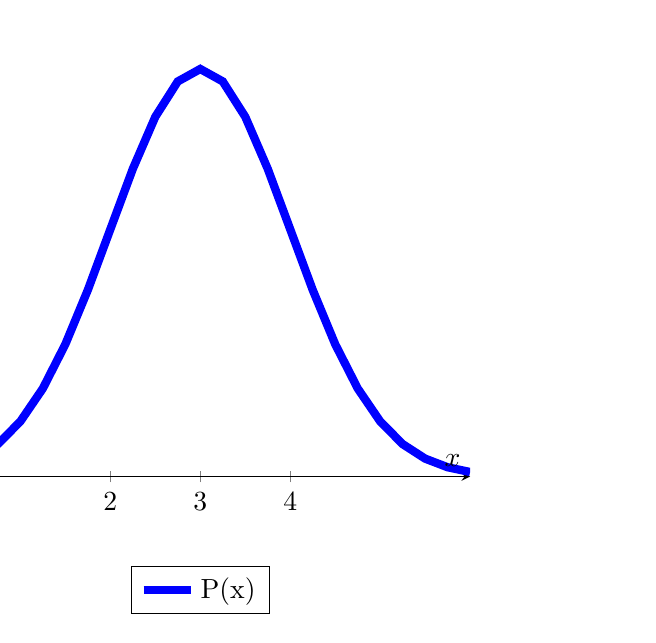
\begin{tikzpicture}
                \hspace*{-2cm}
                	\begin{axis}[
                        axis lines=middle,
                        xlabel=$x$,
                        ylabel=$y$,
                        xtick={0, 2, 3, 4}, % Označení na ose x
                        ytick={ 0, 0.5, 0.8, 1}, % Označení na ose y
                        legend style={at={(0.5,-0.2)}, anchor=north},
                        xmin=0, xmax=6, 
                        ymin=0, ymax=1.1,
                    ]
                    
                    \addplot[blue, domain=0:6, line width = 3pt] {exp(-(x-3)^2/2)};
                    \addlegendentry{P(x)}


                	\end{axis}
                \end{tikzpicture}
            }
\end{graph}



\section{Fuzzy logick\'e spojky}
Fuzzy logické spojky n\'am umožňují vyjádřit vágnost a neurčitost v logických operacích. Tyto spojky se často využívají v aplikacích jako jsou řízení průmyslových procesů, rozpoznávání vzorů, vývoj umělé inteligence a dalších oblastech, kde je potřeba pracovat s neurčitými informacemi.\\

V\v sechny fuzzy logick\'e spojky jsou monot\'onn\'im roz\v s\'i\v ren\'im klasick\'ych logick\'ych spojek. Na dalších kapitolách budou postupně představeny základní fuzzy spojky, mezi kter\'e  patří 
fuzzy negace, konjunkce, disjunkcie a implikace. 

\subsection{Fuzzy negace}

Fuzzy negace představují klíčový koncept v oblasti fuzzy logiky. Tyto negace jsou zobecn\v en\'im klasick\'ych negac\'i. Základní vlastnosti fuzzy negací jsou:

\begin{enumerate}
\item \textbf{Soudržnost:}\\
Pro hodnoty $0$ a $1$ se fuzzy negace shoduje s klasickou negac\'i.
    \item \textbf{Kontinuita hodnot:} \\
        Fuzzy negace nepracuje jenom s  ostrými hodnotami „pravda“ a „nepravda“, ale na stupni neurčitosti či specifickým číselném zápisu, který reflektuje stupeň nepravdivosti.
    \item \textbf{Monotonie:} \\
        Fuzzy negace jsou monot\'onn\'im roz\v s\'i\v ren\'im klasick\'e negace, což znamená, že s rostoucími vstupn\'imi hodnotami klesaj\'i hodnoty výstupn\'e.
    
\end{enumerate}

\begin{definition}
\cite{Kolo} Fuzzy negací nazýváme každou funkci $N:[0, 1] \to [0, 1]$  s vlastnostmi:
    \begin{enumerate}
        \item  $N(0) = 1, N(1) = 0,$
        \item $\forall  x, y \in [0, 1]: x < y \Rightarrow{} N(x) \geq N(y).$
     \end{enumerate}
\end{definition}
     \begin{example}
         Funkce $N_S(x)=1-x$ spl\v nuje vlastnosti fuzzy negace na intervalu $[0,1].$ Je to nejzn\'am\v ej\v s\'i fuzzy negace, kterou ve sv\'e pr\'aci p\v redstavil Lotfi A. Zadeh a obvykle je ozna\v cov\'ana jako standardn\'i negace.   Fuzzy negace nemus\'i b\'yt nutn\v e spojit\'a funkce. Zn\'am\'e p\v r\'iklady nespojit\'ych fuzzy negac\'i jsou n\'asleduj\'ic\'i funkce:
         $$ N_{\bot}(x)=\begin{cases} 1, & \mbox{pokud }x=0 \\ 0, & 
         \mbox{pokud }x\in \mbox{]0, 1]} \end{cases}, 
         N_{\top}(x)=\begin{cases} 1, & \mbox{pokud }x\in \mbox{[0, 1[} \\ 0, & 
         \mbox{pokud }x=1 \end{cases}.$$
         Funkce $N_{\bot}$ je nejmen\v s\'i a funkce $N_{\top}$ je nejv\v et\v s\'i fuzzy negace, proto
         \begin{equation}
        N_{\bot}(x) \geq N(x) \geq N_\top(x)  \mbox{ pro každé } x \in [0, 1]. \
    \end{equation}
    V literatu\v re jsou negace $N_\bot, N_\top$ zn\'am\'e jako Gödelovy fuzzy negace.
    
    Funkce $N_1(x) = \sqrt{1-x}$ a $N_2(x) = \sqrt{1-x^2}$ jsou zřejmě pro $ x \in [0,1]$ nerostoucí a tak\'e plat\'i:
        \begin{enumerate}
            \item $N_1(0) = \sqrt{1-0} = 1, 
                    N_1(1) = \sqrt{1-1} = 0, $
            \item $N_2(0) = \sqrt{1-0^2} = 1,
                    N_2(1) = \sqrt{1-1^2} = 0.$
        \end{enumerate}
         Tedy i tyto funkce jsou fuzzy negace.

         \begin{graph} Grafy dříve zmíněných funkcí $N_s$, $N_{\bot}$,$ N_{\top}$, $N_1$ a $N_2.$\\
            \resizebox{150pt}{!}{%zde se meni velikost grafu
                \begin{tikzpicture}
                \hspace*{-2cm}
                	\begin{axis}[
                        axis lines=middle,
                        xlabel=$x$,
                        ylabel=$y$,
                        xmin=0, xmax=1.1, 
                        ymin=0, ymax=1.1, 
                        legend entries={$N_s$ = $1-x$},
                        legend style={at={(0.5,-0.2)}, anchor=north}
                    ]
                		\addplot[samples = 500,
                            	smooth,
                            	ultra thick,
                            	blue,] {1-x};
    
                	\end{axis}
                \end{tikzpicture}
            }
            \resizebox{150pt}{!}{%zde se meni velikost grafu
                \begin{tikzpicture}
                \hspace*{-1cm}
                	\begin{axis}[
                        axis lines=middle,
                        xlabel=$x$,
                        ylabel=$y$,
                        xmin=0, xmax=1.1, 
                        ymin=0, ymax=1.1, 
                        %xtick={-1,0,1,2},
                        %ytick={-0.5,0,1,1.5},
                        legend entries={$N_{\bot}(x)$},
                        legend style={at={(0.5,-0.2)}, anchor=north}
                    ]
                    
                    % Prvý prípad: g(x) = 1 pre x = 0
                    \addplot[blue, mark=*] coordinates {(0, 1)};
                    
                    % Druhý prípad: g(x) = 0 pre 0 < x < 1
                    \addplot[blue, domain=0:1, samples=100, line width = 3pt,] {0};

                    \addplot[only marks, mark=*, mark size=3pt, mark options={fill=white}] coordinates {(0, 0)};
    
                	\end{axis}
                \end{tikzpicture}
            }
            \resizebox{150pt}{!}{%zde se meni velikost grafu
                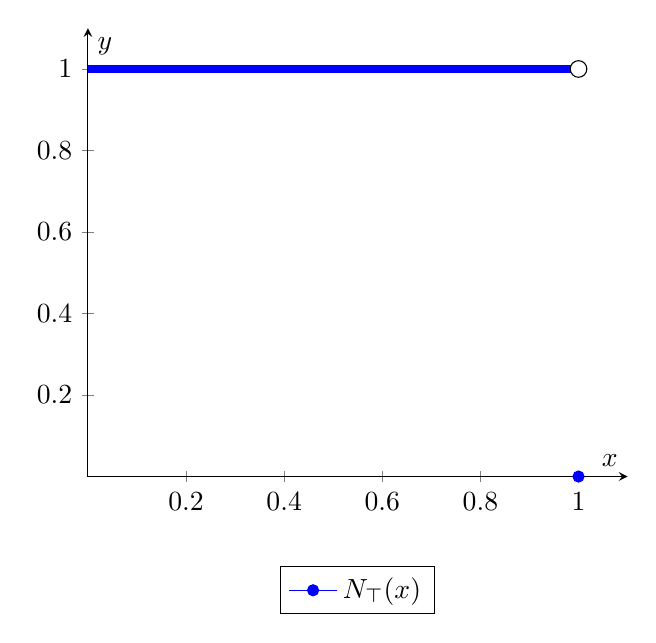
\begin{tikzpicture}
                \hspace*{0cm}
                	\begin{axis}[
                        axis lines=middle,
                        xlabel=$x$,
                        ylabel=$y$,
                        xmin=0, xmax=1.1, 
                        ymin=0, ymax=1.1, 
                        %xtick={-1,0,1,2},
                        %ytick={-0.5,0,1,1.5},
                        legend entries={$N_{\top}(x)$},
                        legend style={at={(0.5,-0.2)}, anchor=north}
                    ]
                    
                    % Prvý prípad: g(x) = 1 pre x = 0
                    \addplot[blue, mark=*] coordinates {(1, 0)};
                    
                    % Druhý prípad: g(x) = 0 pre 0 < x < 1
                    \addplot[blue, domain=0:1, samples=100, line width = 3pt,] {1};

                    \addplot[only marks, mark=*, mark size=3pt, mark options={fill=white}] coordinates {(1, 1)};
    
                	\end{axis}
                \end{tikzpicture}
            }

            \resizebox{150pt}{!}{%zde se meni velikost grafu
                \begin{tikzpicture}
                \hspace*{2cm}
                	\begin{axis}[
                        axis lines=middle,
                        xlabel=$x$,
                        ylabel=$y$,
                        xmin=0, xmax=1.1, 
                        ymin=0, ymax=1.1, 
                        %xtick={-1,0,1,2},
                        %ytick={-0.5,0,1,1.5},
                        legend entries={$N_1$ = $\sqrt{1-x}$},
                        legend style={at={(0.5,-0.2)}, anchor=north}
                    ]
                	\addplot[samples = 200,
                            domain=0:1,
                        	smooth,
                        	ultra thick,
                        	blue,] {sqrt(1-x)};
    
                    
                	\end{axis}
                \end{tikzpicture}
            }
            \resizebox{175pt}{!}{%zde se meni velikost grafu
                \begin{tikzpicture}
                \hspace*{3cm}
                	\begin{axis}[
                        axis lines=middle,
                        xlabel={$x$},
                        ylabel={$y$},
                        xmin=0, xmax=1.1, 
                        ymin=0, ymax=1.1, 
                        xtick={0,0.2,0.4,0.6,0.8,1},
                        ytick={0,0.2,0.4,0.6,0.8,1},
                        legend entries={$N_2$ = $\sqrt{1-x^2}$},
                        legend style={at={(0.5,-0.2)}, anchor=north}
                    ]
                	\addplot[samples = 200,
                            domain=0:1,
                        	smooth,
                        	ultra thick,
                        	blue,] {sqrt(1-x^2)};
    
                   
                	\end{axis}
                \end{tikzpicture}
            }
        \end{graph}
    \end{example}

   N\v ekter\'e fuzzy negace maj\'i dal\v s\'i zaj\'imav\'e vlastnosti:

    \begin{definition}
    \cite{Kolesarova}
        Kdy\v z $N: [0,1] \to [0,1]$ je klesající a spojitá fuzzy negace, \v r\'ik\'ame, \v ze $N$ je striktní negace.
        Fuzzy negace, která je involutivní, tedy negace, pro kterou plat\'i $N(N(x)) = x $ pro každé $ x \in [0,1]$, se nazývá silná fuzzy negace.
    \end{definition}

    \begin{example}
        Spojit\'e neg\'atory $N_S, N_1, N_2$ z p\v redchoz\'iho p\v rikladu jsou evidetn\v e striktn\'i, proto\v ze jsou ryze monot\'onn\'i. D\'ale plat\'i:
        $$N_S(N_S(x))=1-(1-x)=x, \mbox{pro ka\v zd\'e } x \in [0,1],$$
                $$N_1(N_1)) = N_1(\sqrt{1-x}) = \sqrt{1-\sqrt{1-x}} \neq x, \mbox{ pro každé } x \in ]0,1[,$$ $$N_2(N_2) = N_2(\sqrt{1-x^2}) = \sqrt{1-(\sqrt{1-x^2})^2} = x,
\mbox{pro každé } x \in [0,1].$$
Takže negace $N_S$ a $N_2$ jsou involutivní a tím pádem tak\'e siln\'e negace, naopak
            negace $N_1$ není involutivní, tedy ani siln\'a fuzzy negace.
                
            \end{example}

    \begin{remark}
        Z rovnosti $N(N(x))=x$ plyne pro bijektivn\'i funkce tak\'e rovnost $N(x)=~N^{-1}(x).$ 
         Grafick\'a interpretace  t\'eto rovnosti  pro fuzzy negace je taková, že grafy involutivních fuzzy negací jsou osově souměrné podle osy $y = x$.
        \begin{graph} Ukázka osové souměrnosti bijektivní funkce f(x) = $\sqrt{1-x^2}$ podle osy y = x pro $x \in [0,1]$.\\
            
            \begin{tikzpicture}
            \hspace*{3cm}
            	\begin{axis}[
                        axis lines=middle,
                        xlabel=$x$,
                        ylabel=$y$,
                        xmin=0, xmax=1, 
                        ymin=0, ymax=1, 
                        %xtick={-1,0,1,2},
                        %ytick={-0.5,0,1,1.5},
                        legend entries={$g(x)$},
                        legend style={at={(0.5,-0.2)}, anchor=north}
                    ]
            		\addplot[samples = 500,
                        	smooth,
                        	very thick,
                        	blue,] {sqrt{1-x^2}};
                    \addplot[smooth,
                            	thin,
                            	red,
                            	dashed
                            ]  {x};
                \legend{y = $\sqrt{1-x^2}$, 
                    	y = x
                    }
            	\end{axis}
            \end{tikzpicture}
        \end{graph}
    \end{remark}

    
\subsection{Fuzzy konjunkce}

Fuzzy konkjunkce se využívají pro spojení dvou a více podmínek s ohledem na jejich vágnost a neostrost. Místo výsledného \clqq ano\crqq \space nebo \clqq ne\crqq \space je použita hodnota $x$, $x \in [0,1]$, která reprezentuje, do jaké míry jsou podmínky splněny.  
Základní vlastnosti fuzzy konjunkcí jsou:
\begin{enumerate}
    \item \textbf{Soudržnost:}\\
    Pro hodnoty 0 a 1 se fuzzy konjunkce shoduje s klasickou konjunkcí.
    \item \textbf{Kontinuita hodnot:}\\
    Fuzzy konjunkce nepracuje jenom s  ostrými hodnotami „pravda“ a „nepravda“, ale na stupni neurčitosti či specifickým číselném zápisu, který reflektuje stupeň nepravdivosti.
    \item \textbf{Monotonie:}\\
    Fuzzy konjunkce je monotonní operace, tedy pokud A$\leq$ B$\leq$ C$\leq$ D, pak A$\land$B$\leq$ C$\land$D, což znamená, že s rostoucími vstupními hodnotami rostou i výsledky jejich konjunkce.
\end{enumerate}
\begin{definition}
    \cite{hlinena}
    Neklesající zobrazení C: $[0,1]^2 \rightarrow [0,1]$ se nazývá konjunktor, pokud pro libovolné a,b $\in$ [0,1] platí
    C(a,b) = 0 pokud a = 0, nebo b = 0,
    C(1,1) = 1.
    \end{definition}

\begin{remark}
    Existuje velké množství operátor\r u fuzzy konjunkcí, mezi které patří triangulární normy, minima, Lukasiewiczova T-norma, produktní norma a další. Triangulárním normám je pak věnována celá následující podkapitola.
\end{remark}

\subsection{Triangul\'arn\'i normy} Definicia, priklad, ked tri axiomy funguju a jedna nefunguje, priklad styroch znamych t-noriem (minimum, Luk., sucin, drastic), zname triedy-napr. Frank, Yager atd, pridat vhodne obrazky. Konstrukcie spojitych-len definicia a poznamka, ze su vytvorene len pomocou bijektivnych fcii, ale daju sa konstruovat aj nespojite a preto treba zobecnit pojem inverznej fcie. Nic dalsie zatial netreba, ak budeme potrebovat nejaku spec. vlastnost t-noriem, tak potom pridame. Deadline 25.9.\\


Jak již bylo zmíněno, fuzzy konjunkce mohou být formovány pomocí triangulárních norem, zjednodušeně t-norem. 
\begin{definition}
\cite{hlinena}
    Triangulární norma je binární operace na jednotkovém intervale [0,1], tj. funkce $T: [0,1]^2 \rightarrow [0,1]$ taková, že pro každé $x, y, z \in [0,1]$ jsou splněné následující axiomy:
    \begin{enumerate}
        \item \textbf{Komutativnost:} $T(x,y) = T(y,x)$,
        \item \textbf{Asociativita:} $T(x, T(y, z)) = T(T(x, y), z)$,
        \item \textbf{Monotónnost:} pokud $y \geq z$ pak $T(x, y) \geq T(x, z)$,
        \item \textbf{Okrajová podmínka:} $T(x, 1) = x$.
    \end{enumerate}
\end{definition}

\begin{remark}
    Funkce je t-norma v případě, že spl\v nuje alespo\v n 3 ze 4 axiom\r u popsaných výše.
\end{remark}

\begin{example}
    Funkce $F_1 : [0, 1]^2 \rightarrow [0, 1]$ daná přepisem\\
    $$F_1(x,y) = 13,$$
    spl\v nuje axiomy 1., 2., 3., ale nespl\v nuje axiom 4.\\

    Funkce $F_2 : [0, 1]^2 \rightarrow [0, 1]$ daná přepisem\\
    $$F_2(x,y) = x.y.max(x,y)$$
    spl\v nuje axiomy 1., 3., 4., ale nespl\v nuje axiom 2.\\

    Funkce $F_2 : [0, 1]^2 \rightarrow [0, 1]$ daná přepisem\\
    $$F_2(x,y) = x$$
    spl\v nuje axiomy 2., 3., 4., ale nespl\v nuje axiom 1.\\
    
\end{example}

Mezi základní triangulární normy se řadí minimová, součinová, Łukasiewiczova t-norma a drastický součin.
\begin{definition}
\cite{hlinena}
    \begin{enumerate}
    \item \textbf{Minimová t-norma} $T_M: [0,1]^2 \rightarrow [0,1]$
    $$T_M(x,y) = min(x,y).$$
    \item \textbf{Součinová t-norma} $T_P: [0,1]^2 \rightarrow [0,1]$
    $$T_P(x,y) = x.y.$$
    \item \textbf{Łukasiewiczova t-norma} $T_L: [0,1]^2 \rightarrow [0,1]$
    $$T_L(x,y) = max(x+y-1,0).$$
    \item \textbf{Drastický součin} $T_D: [0,1]^2 \rightarrow [0,1]$
    $$T_D:(x)=\begin{cases} min(x,y), & \mbox{pokud }  max(x,y) = 1\\ 
    0, &  jinak.  \end{cases}$$
\end{enumerate}
\end{definition}

\begin{graph} Minimová t-norma $T_M$, Součinová t-norma $T_P$, Łukasiewiczova t-norma $T_L$, Drastický součin $T_D$.\\
   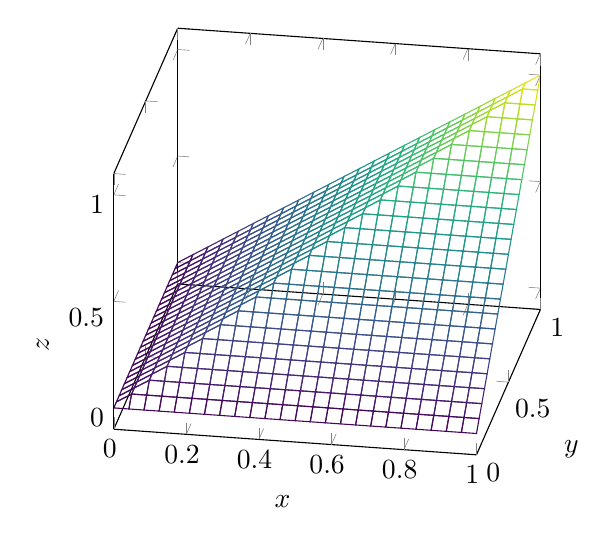
\begin{tikzpicture}
        \begin{axis}[
            width=7cm,  % Nastavte požadovanou šířku grafu
            height=7cm, % Nastavte požadovanou výšku grafu
            xlabel=$x$,
            ylabel=$y$,
            zlabel=$z$, % Popisek osy z
            domain=0:1, % Rozsah hodnot x
            y domain=0:1, % Rozsah hodnot y
            colormap/viridis, % Barevná mapa (nastavitelná)
            view={10}{30}, % Náhled na graf (úhel pohledu)
        ]
        
        % Definice minimove T-normy (minimum z x a y) pomocí gnuplotu
     \addplot3 [surf, shader=interp, mesh] {min(x,y)};
        \end{axis}
    \end{tikzpicture}
    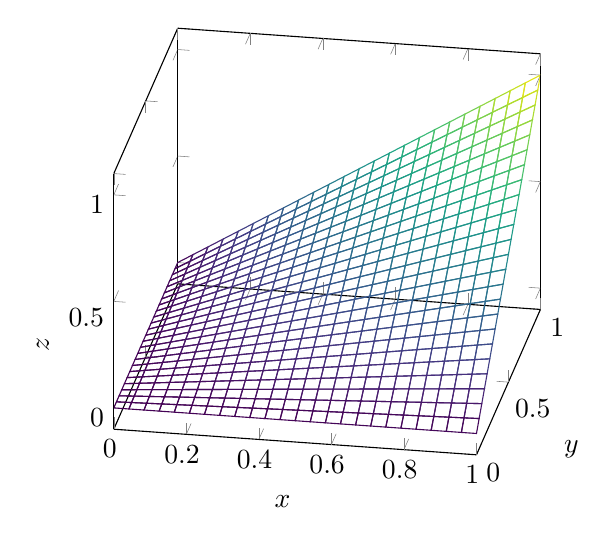
\begin{tikzpicture}
        \begin{axis}[
            width=7cm,  % Nastavte požadovanou šířku grafu
            height=7cm, % Nastavte požadovanou výšku grafu
            xlabel=$x$,
            ylabel=$y$,
            zlabel=$z$, % Popisek osy z
            domain=0:1, % Rozsah hodnot x
            y domain=0:1, % Rozsah hodnot y
            colormap/viridis, % Barevná mapa (nastavitelná)
            view={10}{30}, % Náhled na graf (úhel pohledu)
        ]
        
        % Definice minimove T-normy (minimum z x a y) pomocí gnuplotu
     \addplot3 [surf, shader=interp, mesh] {x*y};
        \end{axis}
    \end{tikzpicture}\\
    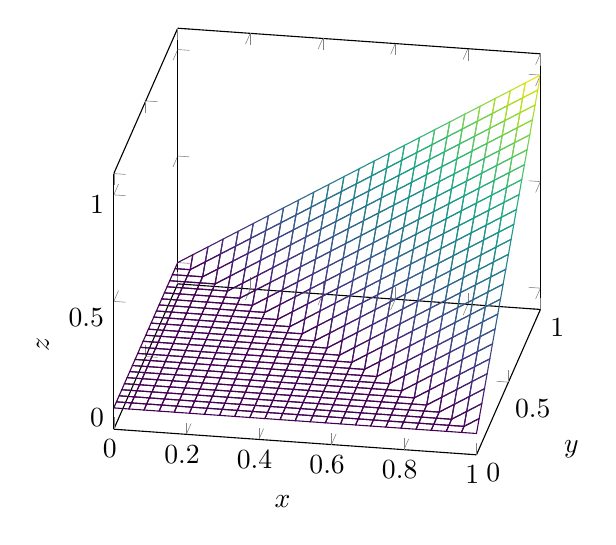
\begin{tikzpicture}
        \begin{axis}[
            width=7cm,  % Nastavte požadovanou šířku grafu
            height=7cm, % Nastavte požadovanou výšku grafu
            xlabel=$x$,
            ylabel=$y$,
            zlabel=$z$, % Popisek osy z
            domain=0:1, % Rozsah hodnot x
            y domain=0:1, % Rozsah hodnot y
            colormap/viridis, % Barevná mapa (nastavitelná)
            view={10}{30}, % Náhled na graf (úhel pohledu)
        ]
        
        % Definice minimove T-normy (minimum z x a y) pomocí gnuplotu
     \addplot3 [surf, shader=interp, mesh] {max(x+y-1,0)};
        \end{axis}
    \end{tikzpicture}
    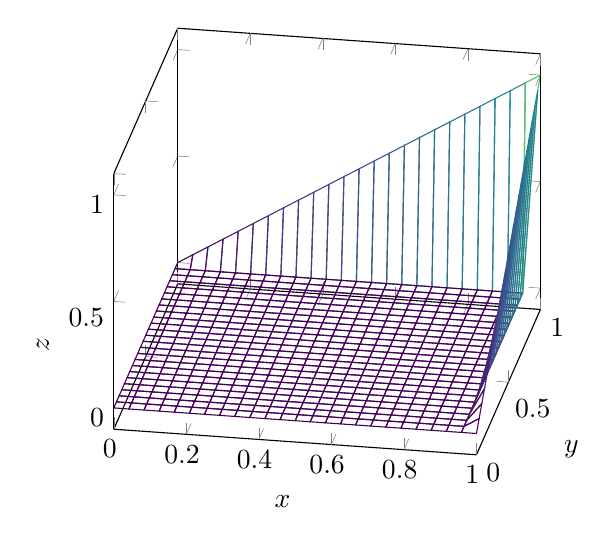
\begin{tikzpicture}
        \begin{axis}[
            width=7cm,  % Nastavte požadovanou šířku grafu
            height=7cm, % Nastavte požadovanou výšku grafu
            xlabel=$x$,
            ylabel=$y$,
            zlabel=$z$, % Popisek osy z
            domain=0:1, % Rozsah hodnot x
            y domain=0:1, % Rozsah hodnot y
            colormap/viridis, % Barevná mapa (nastavitelná)
            view={10}{30}, % Náhled na graf (úhel pohledu)
        ]
        
        % Definice minimove T-normy (minimum z x a y) pomocí gnuplotu
     \addplot3 [surf, shader=interp, mesh] {
                ifthenelse(max(x, y) == 1, min(x, y), 0)
                };
        \end{axis}
    \end{tikzpicture}
    
\end{graph}

\subsection{Pseudoinverzn\'i funkce} Info o tom, ze konstrukcie t-noriem sa daju aj bez pouzitia bijekcii, ale treba zovseobecnenie pseudoinverzu-takze definicia pre neklesajuce, pre nerastuce a priklady+obrazky, zhrnutie napr. o skladanie f a $f^{(-1)}$ veta o tom, ako sa daju t-normy pomocou ps. inv. fcii konstruovat-aditivne a multipl. generovanie, pripadne nejake dalsie zname. Deadline 25.9.
\subsection{Fuzzy disjunkce} Podobne ako pri konjunkciach-deadline 2.10
\subsection{Triangul\'arn\'i konormy} Podobne ako pri t-normach-deadline 2.10
\subsection{Fuzzy implikace} Podobne ako pri konjunkciach-tu ale treba uviest hned rozne pristupy, rozne konstrukcie, vratane tych, ktore potom v dalsej kapitole budete studovat. Deadline 9.10.

{\color{red} Toto som sem dala, lebo nieco z toho vyuzijete v uvodoch konjunkcie a disjunkcie: která se používá k vyhodnocení spojení dvou fuzzy množin. Výsledná fuzzy množina se určuje pomocí tzv. t-norem obsahuje hodnoty, které jsou minimum z odpovídajících hodnot ve vstupních množinách. Fuzzy konjunkce odpovídá binární logické konjunkci, ale výsledek je fuzzy množina s hodnotami mezi 0 a 1. Další logická fuzzy spojka se nazývá \textbf{Fuzzy disjunkce (OR)}. Výsledná fuzzy množina se vyhodnocuje pomocí tzv. t-konorem a obsahuje hodnoty, které jsou maximum z odpovídajících hodnot ve vstupních množinách. Stejně jako fuzzy konjunkce, odpovídá binární logické disjunkci, ale výsledek je také fuzzy množina. V neposlední řadě bych chtěla zmínit \textbf{Fuzzy negaci (NOT)}. Fuzzy negace se používá k invertování fuzzy množiny. Liší se ale od binární logické negace tím, že neinvertuje všechny hodnoty na opačné, ale mírně upravuje pravdivostní hodnoty vstupní fuzzy množiny.


\textbf{Vlastnosti idempotence a involutivity} \\
        Pokud má opakovaná aplikace stejných hodnot vždy tentýž výsledek (idempotence) a při dvojí aplikaci se návratová hodnota rovná hodnotě vstupní (involuce), fuzzy negace je tedy idempotentní a involutivní. 
\textbf{Dualita} \\
        Fuzzy negace jsou navrženy tak, aby vytvářely dualitu s fuzzy operací konjunkce. To znamená, že pokud fuzzy operace konjunkce znamená „velmi pravda“, pak by fuzzy negace měly znamenat „velmi nepravda“. }
  \fi
  
  % Kompilace po částech (viz výše, nutno odkomentovat a zakomentovat input výše)
  % Compilation piecewise (see above, it is necessary to uncomment it and comment out input above)
  %\subfile{chapters/projekt-01-uvod-introduction}
  % ...
  %\subfile{chapters/projekt-05-zaver-conclusion}

  % Pouzita literatura / Bibliography
  % ----------------------------------------------
\ifslovak
  \makeatletter
  \def\@openbib@code{\addcontentsline{toc}{chapter}{Literatúra}}
  \makeatother
  \bibliographystyle{bib-styles/Pysny/skplain}
\else
  \ifczech
    \makeatletter
    \def\@openbib@code{\addcontentsline{toc}{chapter}{Literatura}}
    \makeatother
    \bibliographystyle{bib-styles/Pysny/czplain}
  \else 
    \makeatletter
    \def\@openbib@code{\addcontentsline{toc}{chapter}{Bibliography}}
    \makeatother
    \bibliographystyle{bib-styles/Pysny/enplain}
  %  \bibliographystyle{alpha}
  \fi
\fi
  \begin{flushleft}
  \bibliography{projekt-20-literatura-bibliography}
  \end{flushleft}

  % vynechani stranky v oboustrannem rezimu
  % Skip the page in the two-sided mode
  \iftwoside
    \cleardoublepage
  \fi

  % Prilohy / Appendices
  % ---------------------------------------------
  \appendix
\ifczech
  \renewcommand{\appendixpagename}{Přílohy}
  \renewcommand{\appendixtocname}{Přílohy}
  \renewcommand{\appendixname}{Příloha}
\fi
\ifslovak
  \renewcommand{\appendixpagename}{Prílohy}
  \renewcommand{\appendixtocname}{Prílohy}
  \renewcommand{\appendixname}{Príloha}
\fi
%  \appendixpage

% vynechani stranky v oboustrannem rezimu
% Skip the page in the two-sided mode
%\iftwoside
%  \cleardoublepage
%\fi
  
\ifslovak
%  \section*{Zoznam príloh}
%  \addcontentsline{toc}{section}{Zoznam príloh}
\else
  \ifczech
%    \section*{Seznam příloh}
%    \addcontentsline{toc}{section}{Seznam příloh}
  \else
%    \section*{List of Appendices}
%    \addcontentsline{toc}{section}{List of Appendices}
  \fi
\fi
  \startcontents[chapters]
  \setlength{\parskip}{0pt} 
  % seznam příloh / list of appendices
  % \printcontents[chapters]{l}{0}{\setcounter{tocdepth}{2}}
  
  \ifODSAZ
    \setlength{\parskip}{0.5\bigskipamount}
  \else
    \setlength{\parskip}{0pt}
  \fi
  
  % vynechani stranky v oboustrannem rezimu
  \iftwoside
    \cleardoublepage
  \fi
  
  % Přílohy / Appendices
  \ifenglish
    \input{projekt-30-prilohy-appendices-en}
  \else
    \chapter{Obsah přiloženého pamě\v tového média}

Přiložené CD obsahuje:
\begin{itemize}
  \item \texttt{bp\_xjirmu03.pdf} -- text písemné zprávy ve formátutu PDF
  \item \texttt{tex/} -- zdrojové k\' ody písemné zprávy ve formátu \LaTeX
  \item \texttt{approx/} -- zdrojové k\' ody programu pro aproximaci aditivních generátor\r u
  \item \texttt{questionnaire/} -- zdrojové k\' ody dotazníkového programu
  \item \texttt{README.txt} -- popis jednotlivých částí média
\end{itemize}
  \fi
  
  % Kompilace po částech (viz výše, nutno odkomentovat)
  % Compilation piecewise (see above, it is necessary to uncomment it)
  %\subfile{projekt-30-prilohy-appendices}
  
\end{document}
